\documentclass[tikz,crop,border=4pt]{standalone}
\usepackage{bm}

\definecolor{myred}{RGB}{160,0,0}
\definecolor{mygreen}{RGB}{0,128,0}

\tikzset{
  bitbox/.style={
    draw,
    thick,
    minimum width=\boxsize,
    minimum height=\boxsize,
  },
  emptybitbox/.style={
    bitbox,
    dashed
  },
  leakingbitbox/.style={
    bitbox,
    rotate=24,
    fill=blue!20!white,
  }
}

\newcommand{\bit}[2]{%
  \node[bitbox] at (#1*\boxsize,0) {\textcolor{myred}{\textbf{#2}}};
}

\newcommand{\emptybit}[1]{%
  \node[emptybitbox] at (#1*\boxsize,0) {};
}

\newcommand{\leakingbit}[2]{%
  \node[leakingbitbox] at (#1*\boxsize,-0.48) {\textcolor{myred}{\textbf{#2}}};
}

\begin{document}

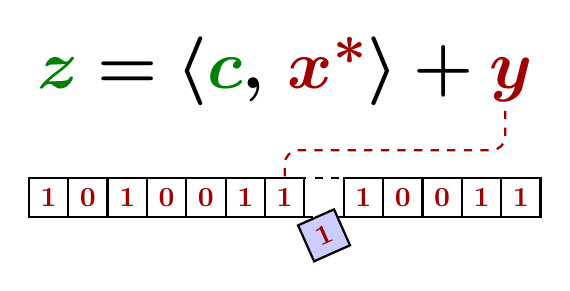
\begin{tikzpicture}[>=stealth]

\node at (0,0)
  {\Huge $\textcolor{mygreen}{\bm{z}} \bm{=} \bm{\langle}
  \textcolor{mygreen}{\bm{c}}\bm{,}\,
  \textcolor{myred}{\bm{x^\ast}}
  \bm{\rangle} \bm{+} \textcolor{myred}{\bm{y}}$};

\draw[draw=myred, dashed, thick, rounded corners=5pt]
  (2.8,-0.5) -- ++(0,-0.5) -- ++(-2.8,0) -- ++(0,-0.4);

\begin{scope}[shift={(-1,-1.6)}]
  \def\boxsize{0.5cm}

  \emptybit{3}
  \leakingbit{3}{1}

  \bit{-4}{1}
  \bit{-3}{0}
  \bit{-2}{1}
  \bit{-1}{0}
  \bit{0}{0}
  \bit{1}{1}
  \bit{2}{1}
  \bit{4}{1}
  \bit{5}{0}
  \bit{6}{0}
  \bit{7}{1}
  \bit{8}{1}
\end{scope}

\end{tikzpicture}

\end{document}
